\chapter{Objetivos}

Una vez situado el Trabajo Fin de Grado en su contexto vamos a presentar los objetivos que nos marcamos para la realización del mismo. Los objetivos a abordar son tres, los cuáles expongo a continuación.


\section{Conexión con ArDrone 2.0}

JdeRobot tiene aplicaciones  como \emph{introrob\_py} desarrolladas en Python o en C++ que se conectan directamente con el cuadricóptero ArDrone de Parrot. Estas aplicaciones solo se pueden ejecutar bajo un sistema operativo Linux. El objetivo es desarrollar una aplicación que sea capaz de conectarse al drone directamente desde el navegador, de tal manera que la aplicación sea multiplataforma.\\

Esta conexión deberá ser capaz de recoger los datos de los sensores y enviarle las órdenes de movimiento a la vez y en tiempo real.\\


\section{Control del drone a través de WebRTC}

Como objetivo principal del proyecto tenemos que implementar la tecnología WebRTC para teleoperar el drone. La conexión punto a punto deberá realizarse entre el ordenador que realiza la conexión con el cuadricóptero y un segundo ordenador. Durante toda la memoria nos referiremos como ordenador local o par local al mini-ordenador que usaremos para conectarnos al cuadricoptero y el cuál deberá ir a bordo del drone, y ordenador remoto o par remoto al ordenador desde el cuál teleoperaremos el vehículo.\\

La conexión WebRTC será bidireccional, y deberá ser capaz de transportar contenido multimedia y datos. La aplicación deberá usar WebRTC para las cumplir las siguientes funcionalidades:

\begin{itemize}

\item \emph{Visualización de cámara a bordo.} WebRTC tendrá que acceder al hardware conectado al equipo local y obtener un flujo audiovisual de la cámara. Este flujo tendrá que ser también enviado usando la misma tecnología web desde el ordenador localhacia el ordenador remoto.

\item \emph{Sensores de navegación.} Los datos obtenidos de los sensores de navegación del cuadricoptero deberán ser enviados al ordenador remoto donde se visualizaran.

\item \emph{Localización espacial del drone.}La brujula y GPS del cuadricoptero deberán ser recogidas por el ordenador local, y deberán enviarse al ordenador remoto para poder visualizar en este un mapa para tener localizado el vehículo.

\item \emph{Ordenes}. Desde el ordenador remoto deberán enviarse hacia el ordenador local las ordenes dadas para el aterrizaje, despegue, y comandos de movimiento.


\end{itemize}

De manera general, el ordenador local deberá conectarse al drone, recoger datos de los sensores y la cámara y entregarle las órdenes. Por otro lado, deberá ser también un par de la conexión WebRTC, y enviar al par remoto todos los datos recogidos en el drone además de la cámara, y recibir de este las órdenes y entregárselas al drone.\\

El ordenador remoto deberá recibir todos los datos de navegación y la cámara del par local, y por otro lado enviar las órdenes y comandos de movimiento al par local. En la figura \ref{fig:esquemageneral} tenemos un esquema de la estructura general del proyecto.\\

\begin{figure}[htb]
\centering
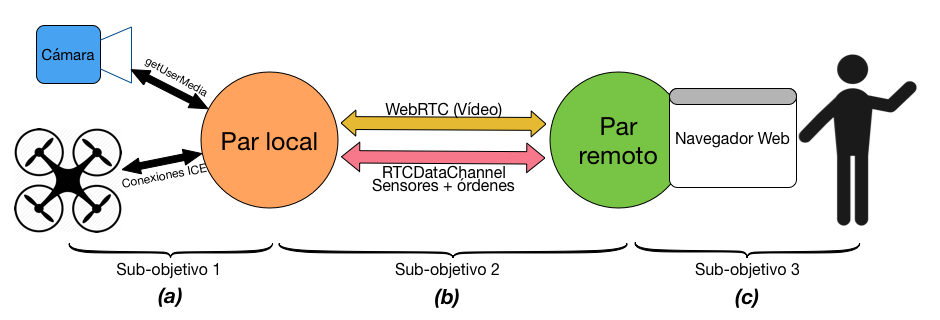
\includegraphics[width=0.9\textwidth]{esquema_general}
\caption{Esquema general del proyecto}
\label{fig:esquemageneral}
\end{figure}

\section{Interfaz amigable y actual}

Uno de los requisitos es desarrollar una interfaz clara, que nos muestre de una manera lo mas realista posible los datos recogidos de los sensores del drone, la cámara, y que tenga unos controles que nos permita manejar el cuadricóptero.\\

Esta interfaz deberá realizarse con tecnología web actual y moderna, y deberá permitirnos el manejo del cuadricóptero de la forma mas realista y similar posible a los sistemas de control de drones que hemos hablado en el capítulo \ref{cap:controldrones}.\\

\section{Metodología y plan de trabajo}

La realización de un proyecto requiere de una metodología que establezca las pautas a seguir y la planificación de las tareas que se deben llevar a cabo para cumplir los objetivos del mismo. Hemos escogido el modelo de \emph{desarrollo en espiral}, ya que es un modelo ampliamente usado en la ingeniería de \emph{software}. Este modelo define una serie de ciclos que se repiten en un bucle hasta el final del proyecto, dividiéndolo en varias subtareas más sencillas y estableciendo puntos de control al final de cada iteración en los que se evalúa el trabajo realizado y se enfocan las nuevas tareas para continuar.\\

Esta metodología recibe su nombre por la forma de espiral que tiene su representación gráfica o diagrama de flujo, que podemos ver en la figura \ref{fig:planificacion_espiral}. En cada iteración se llevan a cabo las siguientes actividades:

\begin{itemize}
 \item \textbf{Determinar los objetivos}, dividir en subobjetivos y fijar requisitos.
 \item \textbf{Analizar los riesgos} y factores que impidan o dificulten el trabajo y las consecuencias negativas que este
 pueda ocasionar.
 \item \textbf{Desarrollar} las tareas para lograr los objetivos según los requisitos especificados.
 \item \textbf{Planificar} las próximas fases tras evaluar el transcurso del proyecto.
\end{itemize}

\begin{figure}[htb]
\centering
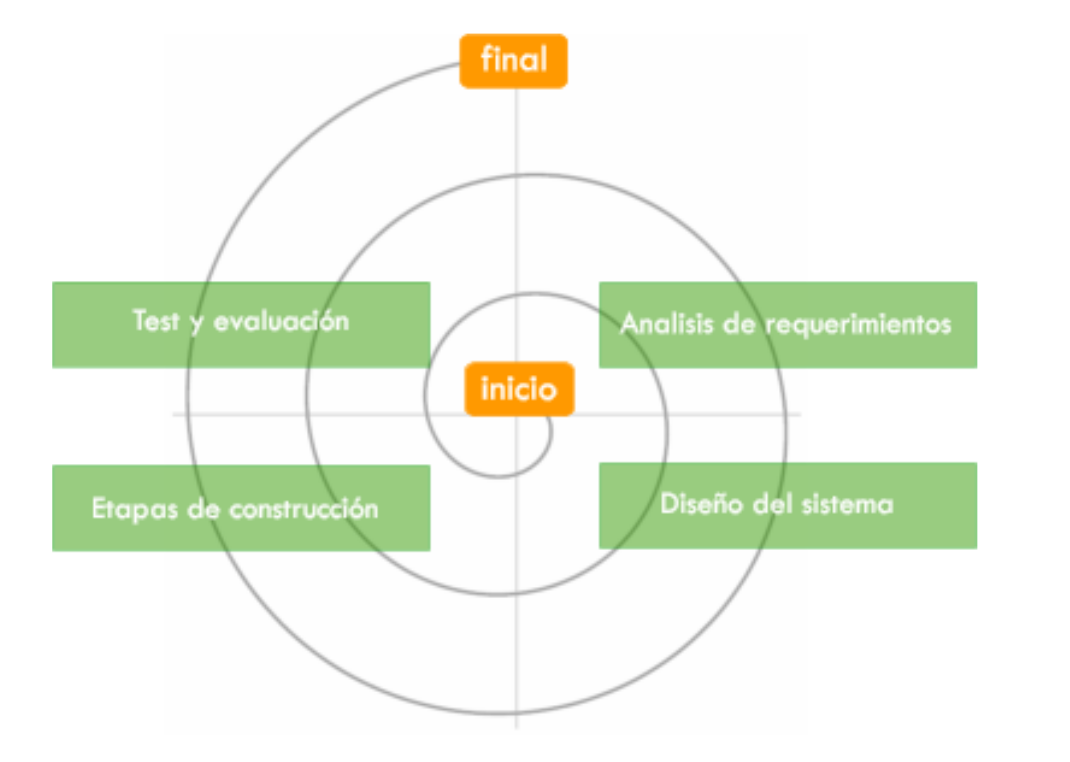
\includegraphics[width=0.9\textwidth]{espiral}
\caption{Esquema general del proyecto}
\label{fig:planificacion_espiral}
\end{figure}

Durante el ciclo de vida del proyecto se han hecho reuniones periódicas con el tutor. En ellas se evaluaban los avances logrados y se marcaba la hoja de ruta a tomar para los siguientes días de desarrollo. Si los puntos marcados en sesiones anteriores no se habian finalizado se ampliaba el plazo o se intentaba buscar otra manera de avance.\\

Para facilitar el seguimiento del proyecto se ha hecho uso de un mediawiki\footnote{http://jderobot.org/Irodmar-tfg} de JdeRobot en el que se iba actualizando cada avance que se lograba, con explicaciones y vídeos e imágenes. Se ha utilizado la plataforma Github\footnote{https://github.com/RoboticsURJC-students/2015-tfg-irodmar}, que es un sistema de control de versiones para alojar el código de todo el proyecto.\\

El plan de trabajo para todo el proyecto se puede dividir en las siguientes etapas:

\begin{itemize}
\item \textbf{Familiarización con JdeRobot}: Primer contacto con esta plataforma y sus herramientas para conocer su funcionamiento.
\item \textbf{Aprendizaje de tecnologías web necesarias:} Conocer las tecnologías web que van a ser necesarias para el desarrollo del proyecto. Entre ellas se encuentra HTML5, CSS3, WebGL, ThreeJS, o jQuery. Primer contacto también con el \emph{middleware} ICE.
\item \textbf{Aprendizaje WebRTC}: Aprendizaje a fondo de esta tecnología web que sera la base del proyecto.
\item \textbf{Desarrollo WebRTC}: Desarrollo de la parte correspondiente a WebRTC dentro de la aplicación.
\item \textbf{Desarrollo uavviwer\_js}: Crear toda la infraestructura necesaria para la interconexión entre el navegador y el drone.
\item \textbf{Desarrollo interfaz}: Desarrollo de la interfaz amigable para teleoperar el drone.
\item \textbf{Experimentos}: Primero se realizan pruebas con el simulador, y cuando el código este suficientemente maduro se prueba con un drone real.
\end{itemize}






